%% This is repurposed from `sample-sigconf.tex'
\documentclass[sigconf,review]{acmart}


\usepackage{graphicx}
\usepackage{hyperref}
\usepackage{cleveref}
\usepackage{tabulary}
\usepackage{soul}
\usepackage{subcaption}
\usepackage{algorithm}
\usepackage{algorithmic}

% pseudocode cpp
\usepackage{listings}
\usepackage{xcolor}


%%
%% \BibTeX command to typeset BibTeX logo in the docs
\AtBeginDocument{%
  \providecommand\BibTeX{{%
    \normalfont B\kern-0.5em{\scshape i\kern-0.25em b}\kern-0.8em\TeX}}}

%% Rights management information.  This information is sent to you
%% when you complete the rights form.  These commands have SAMPLE
%% values in them; it is your responsibility as an author to replace
%% the commands and values with those provided to you when you
%% complete the rights form.
%\setcopyright{acmcopyright}
%\copyrightyear{2018}
%\acmYear{2018}
%\acmDOI{10.1145/1122445.1122456}

%% These commands are for a PROCEEDINGS abstract or paper.
\acmConference[The Web Conference 2021]{The Web Conference 2021}{April 19--23, 2021}{Ljubljana, Slovenia}
\acmBooktitle{The Web Conference 2021, April 19--23, 2021, Ljubljana, Slovenia}
%\acmPrice{15.00}
%\acmISBN{978-1-4503-XXXX-X/18/06}



%%%%%%%%%%%%%%%%%%%%%%%%%%%%%%%%%%%%%%%%
% Useful reviewing/feedback annotations
\input{annotations}
%%%%%%%%%%%%%%%%%%%%%%%%%%%%%%%%%%%%%%%%

%%
%% Submission ID.
%% Use this when submitting an article to a sponsored event. You'll
%% receive a unique submission ID from the organizers
%% of the event, and this ID should be used as the parameter to this command.
%%\acmSubmissionID{123-A56-BU3}

%%
%% The majority of ACM publications use numbered citations and
%% references.  The command \citestyle{authoryear} switches to the
%% "author year" style.
%%
%% If you are preparing content for an event
%% sponsored by ACM SIGGRAPH, you must use the "author year" style of
%% citations and references.
%% Uncommenting
%% the next command will enable that style.
%%\citestyle{acmauthoryear}

%%
%% end of the preamble, start of the body of the document source.
\begin{document}

%%
%% The "title" command has an optional parameter,
%% allowing the author to define a "short title" to be used in page headers.
\title[Columbus: Fast, Reliable Co-residence Detection for Lambdas]
{Columbus: Fast, Reliable Co-residence Detection for Lambdas} % 

%%
%% The "author" command and its associated commands are used to define
%% the authors and their affiliations.
%% Of note is the shared affiliation of the first two authors, and the
%% "authornote" and "authornotemark" commands
%% used to denote shared contribution to the research.
%\author{First Last}
%\affiliation{%
%  \institution{UC San Diego}}
%\email{email@ucsd.edu}



%%
%% By default, the full list of authors will be used in the page
%% headers. Often, this list is too long, and will overlap
%% other information printed in the page headers. This command allows
%% the author to define a more concise list
%% of authors' names for this purpose.
%\renewcommand{\shortauthors}{Trovato and Tobin, et al.}

%%
%% The abstract is a short summary of the work to be presented in the
%% article.

\begin{abstract} 

Cloud computing has seen explosive growth and popularity, especially
``serverless'' service modalities, such as AWS lambdas. These services are
lighter-weight and provide more flexibility in scheduling and cost, which
contributes to their popularity, however the security issues associated with
serverless computing is not well understood. In this work, we construct a covert
channel, a means of transmitting data outside of tranditional channels, that is
practical for AWS lambdas.  We extend the work in Wu et. al to utilize the
memory-bus to develop a co-residence detector that is generic, reliable, and
scalable.  This technique performs dynamic neighbor discovery and is incredibly
fast, executing in a matter of seconds. In addition to this protocol for lambda
co-residence detection, we also perform and evaluate a series of measurements
that exemplify the practicality of this approach in a cloud setting. Through
this work, we show that efforts to secure co-residency detection in cloud
providers is not yet complete.

%Cloud computing has seen explosive growth in the past decade. While
%efficient sharing of the underlying server infrastructure among tenants 
%has contributed to this growth, the same principles also open avenues for 
%cross-tenant attacks. Providers like AWS and Azure have 
%traditionally relied on obfuscation of coresidency information 
%to prevent such attacks. However, recent works have repeatedly found
%covert channels that allow for breaking this encapsulation and detecting
%co-residency, prompting the providers to harden isolation on their platforms. 
%In this work, we find yet another such technique for detecting coresidency of 
%cloud instances. Our technique uses a hardware covert channel based on the 
%memory bus, which is more pervasive and harder to fix. 
%We show that this channel can be used to perform reliable co-residence detection 
%% reliable and fast go against each other. just doing reliable is easy, as you can 
%% get 100% reliability by letting it run forever. The challenge is to have 
%% something that is fast and yet reliable. I don't know how to convey that nicely 
%one that is fast enough for detecting coresidency for the ephemeral serverless functions,
%or lambdas. We use our technique to perform co-operative co-residence detection 
%for thousands of AWS lambdas within a few seconds, which could aid attackers in 
%performing DDoS attacks or learn cloud's internal mechanisms. 
%In this paper, we present the technique in detail, evaluate it, 
%and use it to perform a measurement study on
%lambda activity across AWS regions.  Through this work, we hope to motivate the
%need to address this covert channel.
\end{abstract}


%%
%% The code below is generated by the tool at http://dl.acm.org/ccs.cfm.
%% Please copy and paste the code instead of the example below.
%%
\begin{CCSXML}
<ccs2012>
% <concept>
% <concept_id>10002978.10003001.10010777.10011702</concept_id>
% <concept_desc>Security and privacy~Side-channel analysis and countermeasures</concept_desc>
% <concept_significance>300</concept_significance>
% </concept>
<concept>
<concept_id>10002978.10003006.10003007.10003010</concept_id>
<concept_desc>Security and privacy~Virtualization and security</concept_desc>
<concept_significance>300</concept_significance>
</concept>
</ccs2012>
\end{CCSXML}

\ccsdesc[300]{Security and privacy~Side-channel analysis and countermeasures}
\ccsdesc[300]{Security and privacy~Virtualization and security}


%%
%% Keywords. The author(s) should pick words that accurately describe
%% the work being presented. Separate the keywords with commas.
\keywords{cloud, cartography, serverless, coresidency, covert channels}

%% A "teaser" image appears between the author and affiliation
%% information and the body of the document, and typically spans the
%% page. DO WE NEED THIS?
%\begin{teaserfigure}
%  \includegraphics[width=\textwidth]{sampleteaser}
%  \caption{}
%  \label{fig:teaser}
%\end{teaserfigure}

%%
%% This command processes the author and affiliation and title
%% information and builds the first part of the formatted document.
\maketitle

\section{INTRODUCTION}
\label{sec:intro}

% generally coresidence implies getting an attacker VM colocated with 
% a victim VM - we are not doing that 
% rather we are providing a tool for colocating our own apps 
% in particular, we are figuring out with certainty which of our apps 
% are colocated with others
% 1. we can present it as a tool to aid the isolation, placement 
% and scheduling studies as software-based strategies become infeasible
% due to better isolation strategies
% 2. We prove that an attacker can reliably colocate a bunch of its 
% instances which may facilitate her in much more targeted DDos attacks 
% (find some references) 
% 3. (Speculative) figuring out migration strategies of 
% VMs/containers if deployed on a larger scale might aid in coordinated attacks 
% a la power attacks.
% we present technique as our main contribution for now
% a better way would be use this technique to get some interesting 
% new results and present that as the main contribution


%% Paragraph 1: Introduce cloud computing and the problem of cartography
Cloud computing is a fast growing technology that is widely used around the
globe. Major cloud providers like AWS~\cite{awscloud}, Microsoft
Azure~\cite{azurecloud} and Google Cloud~\cite{googlecloud} provide a multitude
of compute and storage services and have seen immense growth over the past
decade. While there are many benefits of using cloud services, like
increased scalability and decreased IT costs~\cite{Armbrust}, the cloud also
creates new security concerns as multiple tenants share the same underlying
physical infrastructure. For example, by multiplexing applications from multiple
tenants on the same server, cloud computing opens up new avenues and
opportunities for cross-tenant or side-channel attacks through shared server 
hardware like caches~\cite{meltdown, xuccsw2011}. 
While the virtualization platforms used to
share the infrastructure have been constantly improving to harden the isolation
between the tenants, this process is not flawless and usually comes at the 
cost of performance\amirian{better?}\todo{cite}.


% Why another coresidence detection technique
Traditionally, clouds have relied on hiding their placement mechanisms (i.e.,
how they pack tenants onto servers) and co-residence information (i.e., which
particular tenants are placed together on a server) as a first line of defense
against targeted attacks. By reducing an attacker's ability to identify and
target the same server as their victim, attackers may have to execute
brute-force mechanisms that can become expensive with low yield. However, a plethora of
previous work, started by Ristenpart et al.~\cite{ristenpartccs2009}, have
exploited various covert channels to break this encapuslation and 
achieve co-residency detection on clouds
like AWS. These studies then used these channels to demonstrate targeted attacks
or shed light on cloud's internal placement and resource allocation
mechanisms\todo{cite}, which further weaken the cloud encapsulation model. Cloud
providers have since promptly fixed many of these covert channels and produced
solutions (e.g. containers) that provide better isolation, like AWS
Firecracker\cite{firecracker}. However, we find that these encapsulations remain
imperfect.


% What's special about our technique
In this work, we find yet another co-residence detection mechanism among cloud
instances by utilizing the memory bus hardware, first introduced by Wu et.
al~\cite{wuusenix2012}. Our mechanism is generic, reliable 
and scalable, making it useful for co-residence detection in a wide range of 
scenarios, including on different clouds and with a variety of cloud services.
Unlike software-based covert channels that can be fixed with new releases, 
the memory bus channel is inherent to x86 hardware and is harder to fix.  
Moreover, being a hardware-based channel, it is more pervasive--we find that it is
omni-present on all major cloud providers--, and accessible to different kinds of 
(software-based) containers (e.g., virtual machines, serverless functions, etc). 
However, while the hardware presents a binary symmetric channel with minimal 
noise, communicating data reliably through this channel from software is 
complicated by processor scheduling (due to which processes only get random 
intermittent access to the channel), and other software mechanisms that 
introduce noise. In absence of continuous access to the channel, we propose a 
novel sampling-based approach for reliable communication of information 
across the channel. We show that such reliable communication is key to 
scaling the co-residence detection to thousands of cloud instances, which 
is significantly higher compared to previous approaches~\cite{varadarajan2015}.

% Why lambdas
In this paper, we focus on serverless functions, which have experienced an
increased interest and growth in recent years, but also come with their own
unique challenges for coresidence detection. Due to their popularity 
(with flexibility in scheduling and low overhead), 
most cloud services now provide these serverless functions to
developers; AWS calls these serverless functions lambdas~\cite{awslambda} while
GCP refers to them as cloud functions~\cite{gcpfunctions}\footnote{Note that in
this work, we use the terms lambdas, serverless functions, and cloud instances
interchangeably hereafter}.  While the flexibility and low overhead are
attributes that appeal to developers, the converse is that information about
lambda placement is not readily available, and lambdas have restricted runtimes
that limit low-level code often used in co-residency detection, making
co-residence detection more difficult. Moreover, lambdas are also more ephemeral
(running for a maximum of 15 minutes on AWS for example), 
forcing any potential co-residence
detection to be faster than previously known mechanisms. 

%\amirian{this sentence feels awkward}Since other
%tradition containers are less restrictive, lambda co-location detection can be
%replicated easily in these other environments.

% Summary of what we did
We only focus on \emph{cooperative} coresidence detection, where all the 
lambdas are assumed to be in adversary's control. Such co-residence 
detection can aid the adversary in many ways. It be used to learn cloud's 
internal placement and resource scheduling mechanisms that may aid an attacker 
in targeted attacks\cite{ristenpartccs2009,varadarajan2015}. It could help 
attacker pack many instances on the same server to perform DDoS attacks. 
Moreover, such mechanism aids in studying performance isolation and other 
such service guarantees of a cloud using colocated instances\cite{wangusenix2018}.
For such cooperative co-residence detection, we propose a neighbor discovery 
protocol using which the co-resided lambdas discover each other. 
We demonstrate the colocation with 100\% success rate for (bigger) lambdas 
and furthermore, we can acheive this within a minute for thousands of them.
Finally, we also perform a measurement study on colocation patterns in
various AWS regions with some insights on lambda activity. \todo{add more
concrete takeaways} Through this, we hope to motivate the need to address the
memory bus covert channel in all the three clouds, and prove that encapsulation
is an ever changing landscape.


% Organization
The remainder of this paper is organized as follows. Section
\ref{sec:background} presents some background from the literature. Sections
\ref{sec:methodology} and \ref{sec:technique} present our co-residence detection
mechanism in detail. We evaluate the mechanism in section \ref{sec:eval} and
conclude with a placement study of AWS lambdas using our technique in section
\ref{sec:study}.  

\section{Background}
\label{sec:background}

We begin with a brief background on relevant topics.

\subsection{Lambdas/Serverless Functions}
\label{sec:background:lambdas}
\todo{needs sprucing}
One of the fast-growing cloud services in recent years are serverless functions such as lambdas on AWS~\cite{awslambda} and cloud functions on GCP~\cite{gcpfunctions}. This interest stems from the fact that serverless architecture does not require the developer to worry about provisioning, maintaining, and administering servers. Additionally, lambdas are much more cost-efficient than VMs as they allow more efficient packing of the servers. However, these functions are more ephemeral than containers and VMs, in many cases only  few minutes. While this attribute provides more flexibility in cost and functionality, the nature of serverless functions also increases the difficulty in detecting co-residency and launching successful attacks.

We focus on AWS Lambdas in this paper but we show that our study is applicable to other clouds as well. Lambdas execute as much smaller units than containers and virtual machines. Lambda sizes range from 128 MB to 3 GB, and their maximum timeout value is 15 minutes. While lambdas are limited in the computations they can execute, they are conversely incredibly lightweight and can be initiated and deleted in a very short amount of time. Since lambdas are short-lived and lightweight, the user has no control over the physical location of the server(s) on which their lambdas are spawned. 

%This seems like a repeat of similar content in other places in the paper, so I've commented it out for now - AM
%In addition to being a relatively recent addition to the long list of %cloud computing services provided, the seemingly fleeting nature of %Lambdas make it challenging to perform targeted co-location attacks %using hardware channels. This could potentially be the reason why %Lambdas have not been explored as much as virtual machines and %containers in literature. But the same characteristics of Lambdas are %what make them interesting to explore, which is what we set out to do %in this work.

\subsection{Co-residence Detection}
\label{sec:background:pastwork}

%On previous work on colocation, past techniques and why those techniques would 
%not work anymore
To perform side-channel attacks against other tenants in a cloud setting, attackers 
need to co-locate their applications on the same servers as their victims. Past 
research has used various strategies to achieve co-residency for demonstrating 
such attacks. Typically, achieving co-residency includes a (VM/Container) launch 
strategy (varying number of instances, time of the day, etc) combined with a 
co-residence detection mechanism 
for detecting if two instances are running on the same machine. Traditionally, 
this was done based on software runtime information like public/internal IP addresses\cite{ristenpartccs2009}, files in \textit{procfs} or other environment variables\cite{wangusenix2018} and other such logical side-channels\cite{varad191016,vmplacement}
that two instances running on a same server might share. 

As virtualization platforms move towards stronger isolation between instances 
(e.g. AWS' Firecracker VM \cite{firecracker}), these logical side-channels have 
become less effective or infeasible. Furthermore, some of these side-channels were only 
effective on container-based platforms that share the underlying OS image and were 
less suitable for hypervisor-based platforms. This prompted a move 
towards hardware-based covert channels which can bypass software isolation and are usually harder to fix. Typically, these covert channels involve 
sending/receiving information by causing contention on a shared hardware that 
results in observable performance fluctuations across applications. A 
number of such side-/covert channels based on shared hardware like last-level caches \todo{references}, memory bus~\cite{wuusenix2012,zhang2016,varadarajan2015} and 
storage devices\todo{references} have been explored in the past, some 
of which have already been addressed and are no longer even feasible in 
most clouds (e.g., last-level cache-based channels\cite{cache-sidechannels}). 

%  \subsection{Random Number Generator hardware}
%  \label{sec:background:rng}
%  When examining avenues for co-location on lambdas, one avenue we explored is the random number generator (RNG) hardware. Modern processors support a shared hardware module to generate true random numbers. These devices use low level noise signals such as thermal noise and other quantum phenomena to produce true non deterministic entropy. Information from this module is routed from the host machine to the /dev/random file in the guest virtual machine for cryptographic operations. Since the hardware is shared, if one guest consumes these random bits within an infinite loop, another user could notice a spike in random operations, indiciating contention.

% Rdrand and rdseed are the two instructions used to access random bits produced by the RNG generator hardware. The bits in the conditional buffer are directly used by the rdseed instruction, but rdrand uses another deterministic module that depends on the past outputs, which helps rdrand achieve a higher throughput than rdseed. This design makes rdseed more reliable to use as rdseed instructions are easily and quickly exhaustible. 

\subsection{Memory Bus Covert Channel}
\label{sec:background:membus}
One shared hardware that we examine in our study is the memory bus. The memory bus is the piece of hardware that connects the memory controller to main memory. Memory bus contention can be caused by initiating repeated memory accesses to saturate the bus bandwidth and cause observable latency spikes. However, this turns out to be very challenging given the multiple levels of caches on today's servers, which prevent repeated memory accesses, and the high memory bandwidth that cannot be saturated by few CPU cores. 

In x86 systems, atomic memory instructions designed to facilitate multi-processor synchronization are supported by cache coherence protocols as long as the operands stay within a cache line (which is generally the case as language compilers make sure that operands are aligned). However, if the operand is spread across two cache lines (referred to as "exotic" memory operations), x86 hardware achieves atomicity by locking the memory bus to prevent any other memory access operations until the current operation finishes. This
 results in significantly higher latencies for the other operations
 which cannot use the ample memory bandwidth due to the lock\cite{wuusenix2012}. Furthermore, this behaviour persists even in the presence of multiple processor sockets, making the locking effects visible to all the cores on the machine. We exploit this property of x86 hardware to cause contention on the memory bus and use the 
 resulting observable variations in performance as a covert channel for detecting co-residency. 

% \section{Motivation}
% \label{sec:motivation}

% % Does adding a threat model section make sense?
% \amirian{Given the intro, I think we can safely remove this section. I've tried to work in pertinent parts into the intro}

% % but whatever works for lambdas is applicable to containers & VMs...
% % can we definitively say this?

\section{Methodology}
\label{sec:methodology}

% TODO: This figure shows only mem access latencies of exotic 
% operation. how does these operations affect latencies of other exotic 
% operations or regular memory accesses?
\begin{figure*}[h!]
\begin{subfigure}{.33\textwidth}
  \centering
  \includegraphics[width=.99\linewidth]{fig/membus_aws.pdf}
%   \caption{1a}
%   \label{fig:sfig1}
\end{subfigure}%
\begin{subfigure}{.33\textwidth}
  \centering
  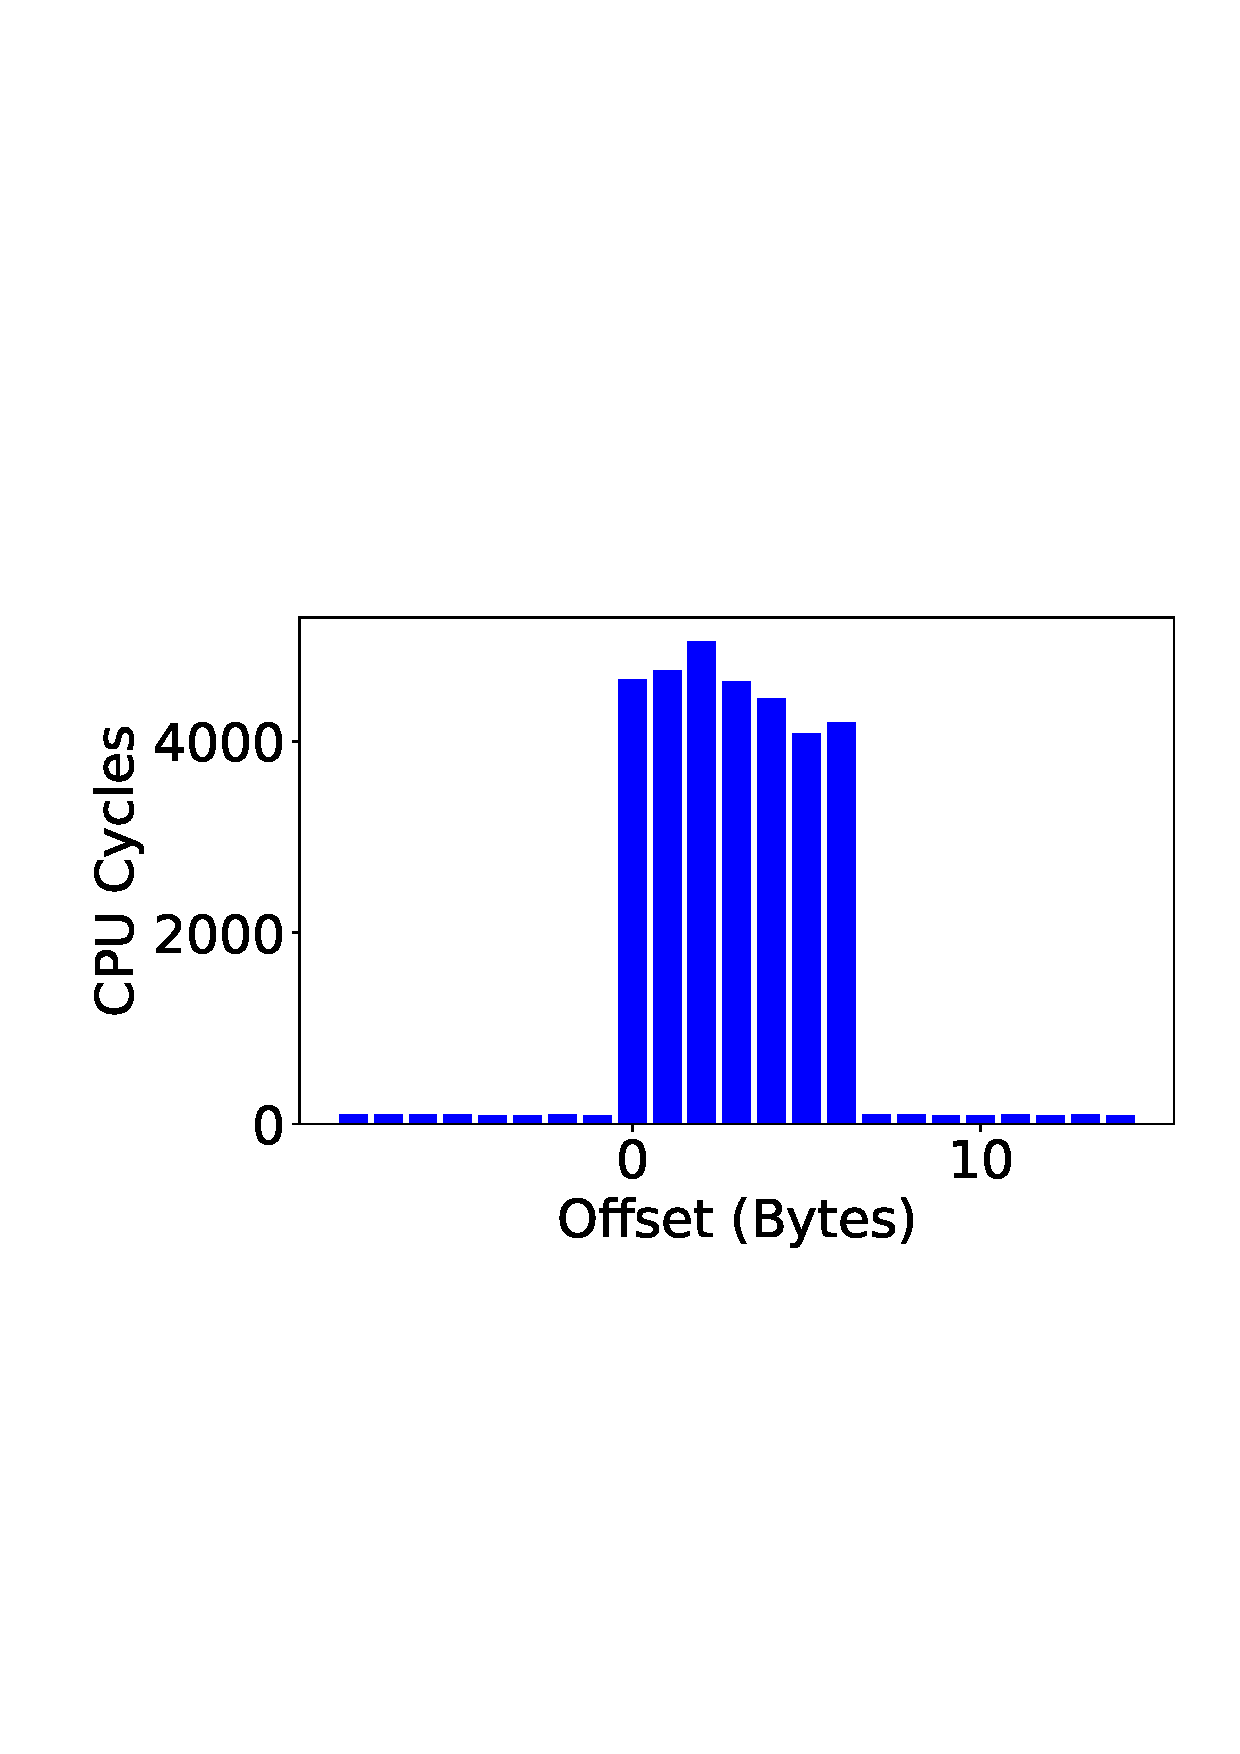
\includegraphics[width=.99\linewidth]{fig/membus_azure.pdf}
%   \caption{1b}
%   \label{fig:sfig2}
\end{subfigure}
\begin{subfigure}{.33\textwidth}
  \centering
  \includegraphics[width=.99\linewidth]{fig/membus_gcp.pdf}
%   \caption{1b}
%   \label{fig:sfig2}
\end{subfigure}
\caption{From left to right, the plots show the latencies of atomic 
      memory operations performed on an 8B memory region as we slide it 
      from one cache line across the boundary into another, on AWS, Azure and 
      Google (GCP) clouds respectively. The latencies 
      are orders of magnitude higher when the 8B region falls across the 
      two cache lines (offsets 0-7B) demonstrating the presence of 
      the memory bus covert channel on all these clouds. \label{fig:membus_clouds}}
\label{fig:fig}
\end{figure*}


Our goal is to determine a (co-operative) co-residence detection mechanism for
lambdas. In other words, given a series of spawned lambdas in a
given region on a cloud service, how can we determine the lambdas that are
co-located on the same machines?  In this section, we discuss the details of
such a mechanism, previous solutions to this problem, and the unique challenges
we faced with lambda co-residence.

Given a set of cloud instances (VMs, Containers, Functions, etc) deployed
to a public cloud, a co-residence detection mechanism would identify, for each 
pair of instances in the set, whether the pair was running on the same physical 
server at some point. Paraphrasing Varadarajan et al.\cite{varadarajan2015}, for 
any such mechanism to be useful across a wide range of 
launch strategies, we observe that it should have the following desirable 
properties:

\begin{itemize}
    \item \textbf{Generic} The technique should be applicable across a wide
    range of server architectures and software runtimes. In practice, the
    technique would work across most third-party clouds and even among different
    platforms within a cloud.
    \item \textbf{Reliable} The technique should have a reasonable detection success
    with minimal false negatives (co-resident instances not detected) and even 
    less false positives (non co-resident instances categorized as co-resident).
    \item \textbf{Scalable} A launch strategy may require hundreds or even thousands 
    of instances to be deployed, and must scalable such that the 
    technique will take less time to detect all co-resided pairs at a reasonable cost.
\end{itemize}

\noindent We add another property to that list which is relevant to lambdas:
\begin{itemize}
    \item \textbf{Fast} The technique should be fast, preferably finishing in 
    the order of seconds. As lambdas are ephemeral (with some clouds restricting their 
    execution times to as low as a minute), the technique should leave ample time 
    for other activities that make use of the resulting co-resident information.
\end{itemize}


Given these properties, we decide to investigate harware-based covert channels.
Hardware-based covert-channels are more difficult to remove and obfuscate than
software-based covert channels, and are also more ubiquitous, given that
hardware is more homogenous in nature than software. 
% generic

% \subsubsection{RNG Hardware}
% \amirian{This feels a bit awkward. We might want to move this to discussion}
% We first examined covert channels based on Random Number Generator (RNG)
% hardware\cite{evtyushkinccs2016}.  Modern processors support this shared
% hardware module to generate true random numbers. 
% % These devices use low level noise signals such as thermal noise and other
% % quantum phenomena to produce true non deterministic entropy. 
% To produce true random numbers, information from this module is routed from the
% host machine to the /dev/random file in the guest virtual machine for
% cryptographic operations. Since the hardware is shared, if one guest consumes
% these random bits within an infinite\amirian{does it need to be infinite?} loop,
% another user could notice a spike in random operations, indicating contention on
% the machine.
% \amirian{do we have an old graph to back up this point of being too noisy? to
% just drive the point home that RNG is not great for these purposes} 
% However, our experiments on AWS using RNG hardware indicated that this channel
% is unreliable for lambda co-detection. We hypothesize that perhaps, because
% causing contention is easy, the channel gets too noisy as a result to accurately
% use for our purposes.

% In order to get random bits, we used a Python module called rdrand that supports 
% both rdrand and rdseed instructions. While our initial plan was to run only rdseed 
% instructions which seemed better suited for our attacker logic, we found that 
% AWS hosts did not support rdseed. We also observed that rdseed was not supported 
% by few of the hosts on GCP. Hence, we run a unified program that uses rdseed
% when available and falls back on rdrand otherwise.\todo{I think we ended up 
% ditching the rdseed idea and stuck to just rdrand. (confirm just in case)} 

% We ran a simple experiment to determine if RNG techniques would be fruitful 
% for our goals. In the first run, we labeled lambdas as victims or attackers. 
% Victim lambdas would take their first set of measurements, sleep for five seconds, 
% and then take a second set of measurements. Attacker lambdas would sleep for the 
% first six seconds (long enough to allow victims to sample once without possible contention), 
% and then start "attacking". In the second run, we simply had victim lambdas run without 
% any attackers causing possible contention.  We show our results in figure~\todo{add the figure in}, 
% where the red dots are the victim lambdas that executed with the presence of attacker 
% lambdas, and the blue dots are victim lambdas that executed alone. There does not appear 
% to be a significant difference between executions when an attacker does and does not exist, 
% which indicates that RNG hardware might not be a salient avenue for determining 
% lambda co-location, as we are not able to differentiate when contention is happening.

\subsubsection{Memory bus channel}
We chose the memory bus covert channel described in
section~\ref{sec:background:covertchannels} as it exploits a fundamental hardware
vulnerability that is present across all generations of x86 hardware.
Historically, multiple public cloud services have been vulnerable to this
channel~\cite{varad191016,zhang2016}, and we found that they are still
vulnerable today. To demonstrate the presence of the vulnerability, we measure
the latency of atomic operations on a 4B memory region as we slide the region
from one cacheline into another across the cacheline boundary. We perform this
experiment on three major clouds (AWS, Google and Microsoft Azure) and show the
latencies observed in Figure~\ref{fig:membus_clouds}. From the figure, we can
see that all three clouds still exhibit significant difference in latencies for
the "exotic" memory locking operations (where the memory region falls across
cacheline boundary) when compared to regular memory accesses, demonstrating the
presence of this covert channel on all of them. Moreover, we were able to run
these experiments on serverless function instances. Since lambdas have runtimes 
that are generally restricted to high-level languages
(that prevent the pointer arithmetic required to perform these exotic
operations), we used the unsafe environments on these clouds --- C++ on AWS,
Unsafe Go on GCP, Unsafe C\# On Azure. This shows the applicability of using the
covert channel across different kinds of cloud instances as well.


% why previous approaches were not scalable
\subsubsection{Previous approaches}
Previous works that used the memory bus for co-residence detection divide the
deployed instances into sender and receiver roles, and attempt to
colocate the sender role with a receiver role. The sender instances
continually lock the memory bus (locking process) for a certain duration
(\textasciitilde 10 seconds) while the receiver samples the memory for any spike
in access latencies (probing process). If all the deployed instances try the
detection i.e., locking and probing at once, (some of) the receivers may see
locking effects, but there would be no way of knowing which or how many senders
co-resided with a particular receiver and caused the locking. This provides
no information about the number of physical servers that ran these instances or
the amount of co-location. The only information we can deduce is that receivers
were probably co-located with just a single sender.

An alternative method is to try pair-wise detection where only one sender 
instance locks and one victim instance probes at a time revealing co-residence
of this pair, and repeating this serially for each pair. However, this technique
is too slow and scales quadratically with the number of instances e.g., a
hundred instances take more than 10 hours assuming 10 secs for each pair.
Varadarajan et al.\cite{varad191016} speeds up this process significantly by
performing detection for mutually-exclusive subsets in parallel, allowing for
false-positives and later eliminating the false-positives
sequentially\amirian{might want to elaborate on this; on its own may be a bit
confusing}. This would still only scale linearly in the best case, which is
still expensive; with a thousand instances, for example, the whole detection
process takes well over 2 hours to finish, which is infeasible for lambdas that
are, by nature, ephemeral. Thus, one challenge in this work is creating a faster
neighbor detection algorithm.

% how do we scale it - challenges.
\subsubsection{The Path to Scalability}`'

%One challenge in creating a lambda neighbor detection algorithm is speed. - repeated
One method to quicken the co-location process is by decreasing the time a single
sender-receiver pair requires to determine co-residence i.e., improving upon
probing time and accuracy of the receiver.  However, this method only affects
total time by a constant factor. To improve scalability, we need to be able to
run the detection for different sender-receiver pairs in parallel without
sacrificing the certainty of information we get when they are run serially.  For
example, when two pairs observe co-residence, we must be certain that each
receiver experienced co-residence because of its own paired sender instance, which
is not possible if co-residence is ascertained based a simple yes/no signal from
the sender instances. 

Previous work utilized the memory bus channel to exchange more complex
information like keys~\cite{wuusenix2012}. At first sight, it appears that the
memory bus can be used to exchange information, such as unique IDs, between the
co-resided instances, which would allow us to ascertain receiver/sender pairs.
However, the previous work assumes that there is only one sender and one
receiver that know exactly how and when to communicate. As we will see in the
next section, this model is not sustainable when there exist many parties that
have no knowledge of each other but try to communicate on the same channel.

To solve some of the challenges mentioned previously, we propose a protocol in
which we use the memory bus covert channel to exchange information between the
instances that have access to the channel. Using the protocol, co-resided
instances can reliably exchange their unique IDs with each other to discover
their neighbors. The protocol takes time on the order of number of instances
involved, which is limited by the maximum number of co-located instances on a
single server (tens), a number that is orders of magnitude less than total
number of instances deployed to the cloud (hundreds to thousands).  This lets us
scale our co-residence detection significantly, as we will see the the next
section.

\section{Neighbor Discovery Protocol}
\label{sec:technique}
 
As noted earlier, co-residence detection scales well when co-residing 
instances on each server communicate among themselves and discover each other. 
Assuming that the instances 
have unique IDs, this requires the co-resided instances to exchange these (integer) IDs with each other using the memory bus channel as a transmission medium. In this section, we present a communication protocol that the co-resided instances can use to achieve this in a fast and reliable way. We first discuss the challenges we faced in making the 
channel reliable before diving into the protocol itself.

\begin{algorithm}[!t]
\caption{Writing 1-bit from the sender}
\label{alg:sender}
\begin{algorithmic}
\STATE $now \leftarrow  time.now()$
\STATE $end \leftarrow now + sampling\_duration$
\STATE $address \leftarrow cache\_line\_boundary-2$
\WHILE{$now < end$}
    \STATE $\_\_ATOMIC\_FETCH\_ADD(address)$
    \STATE $now \leftarrow  time.now()$
\ENDWHILE
\end{algorithmic}
\end{algorithm}

\subsection{Reliable Transmission}
Consider the simple scenario where there is one sender and one receiver 
instance on a machine, and the sender has a set of bits that it needs to communicate 
with the receiver on the memory bus covert channel. On the sender side, to send 
a 1-bit the sender causes contention on the memory bus by locking it using
the special memory locking operations as discussed in section \ref{sec:background:membus} 
(pseudo-code of the sender is shown in Algorithm \ref{alg:sender}).
\todo{what is the subject here? rewrite with subject at front} Reading the bit on a 
receiver would then require sampling the memory bus for contention, 
inferring a 1-bit when the contention is observed or a 0-bit otherwise.

\subsubsection{Sensing contention} 
There are two ways in which the receivers could detect memory bus contention. 
When the memory bus is locked, any non-cached memory 
accesses will queue and therefore see higher latencies. The receiver can 
then continually make un-cached memory accesses (referred to 
as \textit{memory probing} receiver in literature\cite{varadarajan2015}) and 
observe spike in their latencies to detect contention.
The receiver could also use the same memory locking 
operations as the sender (referred to as \textit{memory locking} receiver) to 
probe the memory bus. 
Since only one processor core can lock the memory bus at a given time, any other 
concurrent locking operation will see higher latency. 

Previous studies\cite{wuusenix2012,varadarajan2015} have established that both 
memory probing and locking receivers experience significant latency overhead when compared 
to their baselines during memory bus contention, making both of them desirable 
contenders for sensing the channel on the receiver side. We examine which of the two 
would be more fruitful for our experiments. Memory probing involves regular (un-cached) 
memory accesses, which is universal, unlike the locking operations which are rarely used, 
if at all, by standard applications. This makes memory probing the only viable option 
for non-cooperative co-residence detection, where 
victims are not under attacker's control and cannot be assumed to perform locking 
operations. Furthermore, memory probing can be done on multiple receivers 
constantly without affecting each other (due to the high memory bandwidth), which prevents 
noise in measurements. This is an important attribute, as memory locking receivers 
must contend with this noise. However, bypassing multi-levels of caches in today's servers 
to perform memory accesses with reliable consistency is a challenging task 
\todo{cite some papers}. Even with a reliable cache-bypassing technique, the 
variety of cache architectures and sizes that we encounter on different clouds 
would make tuning the technique to suit these architectures an arduous task while 
reducing the applicability of our overall co-residence detection mechanism. 
Thus, we decide to use the memory locking receiver.


\begin{algorithm}[!t]
\caption{Reading a bit in the receiver}
\label{alg:receiver}
\begin{algorithmic}[1]
\STATE $now \leftarrow  time.now()$
\STATE $end \leftarrow now + sampling\_duration$
\STATE $sampling\_rate \leftarrow num\_samples / sampling\_duration$
\STATE $address \leftarrow cache\_line\_boundary-2$
\STATE $samples \leftarrow \{\} $
\WHILE{$now < end$}
    \STATE $before \leftarrow RDTSC()$
    \STATE $\_\_ATOMIC\_FETCH\_ADD(address)$
    \STATE $after \leftarrow RDTSC()$
    \STATE $samples \leftarrow samples \cup \{(after-before)\}$
    \STATE \textbf{wait until} $NEXT\_POISSON(sampling\_rate)$
    \STATE $now \leftarrow  time.now()$
\ENDWHILE
\STATE $ks\_val \leftarrow KOLMOGOROV\_SMIRINOV(samples, baseline)$
\STATE \textbf{return} $ks\_val < ksvalue\_threshold$
\end{algorithmic}
\end{algorithm}


\subsubsection{Sampling frequency}
Ideally, a memory locking receiver would perform locking operations in a loop and 
look for a dip in the moving average of the number of operations to determine
contention in real-time. Note that, in this case, there is 
essentially no difference between the sender and receiver (i.e., both continually issue
locking operations) except that receiver is taking measurements. This is adequate when 
there is a single sender and receiver~\cite{varadarajan2015},
but when there are multiple receivers, the mere act of sensing the channel by one 
receiver causes contention and other receivers cannot differentiate between a silent (0-bit) 
and a locking (1-bit) sender. To avoid this, we space the sampling of memory bus such that 
no two receivers would sample the bus  at the same time, with high probability. 
We achieve this by using large intervals between successive samples and a poisson-sampling 
to prevent time-locking of receivers. We determined that a millisecond poisson gap between 
samples is reasonable to minimize noise due to collisions in receiver sampling~\ref{fig:membus_clouds}, 
assuming ten co-resided receivers and sampling takes a few microseconds each time.

\subsubsection{Sampling duration}
\label{sec:method:samplingdur}
A receiver can confirm contention with high confidence with only a few samples, assuming 
that the sender is actively causing contention on the memory bus
and the receiver is constantly sampling the memory bus throughout the sampling duration. 
However, in practice, the time-sharing of processors produces difficulties. 
The sender is not continually causing contention, and neither is the receiver sensing it, 
as they are context-switched by the scheduler to run other processes. 
Assuming that the sender and receiver are running on different 
cores, the amount of time they are actively communicating depends on 
the proportion of time they are allocated on each core and how they are 
scheduled. 

To illustrate such behavior, we run a sender-receiver pair using 
the Lambdas\cite{awslambda} of various sizes on AWS,
and compare the distribution of latencies seen by the receiver during the 
contention in each case. Figure \ref{fig:context_switching} shows that the much smaller 
128 MB lambdas (which probably share a CPU core with others and gets constantly context-switched) 
show less active communication than the bigger 3 GB lambdas (which may run on dedicated cores). 
This means that smaller instances that tend to share
processor cores with a lot of other instances may need to pause for more time
and collect more samples to make up for lost communication due to scheduling.
% Since the typical scheduling quantum is on the order of milliseconds, they 
% will need at least a second?


\begin{figure}[!t]
  \includegraphics[width=.99\linewidth]{fig/lambda_sched_effect.pdf}
  \caption{Shows CDF of latencies observed by 128 MB, 1 GB and 3 GB Lambdas during 
  contention. The 128 MB lambda pair sees less contention due to more context switching, 
  whereas the 1 GB and 3 GB lambdas see progressively more contention compared to baseline 
  which we attribute to their relative stability on the underlying physical cores. 
\label{fig:context_switching}}
\end{figure}

\subsubsection{Overcoming noise} 
\label{sec:method:noise}
Along with context switching and sensing noise, there are other imperfections 
in measurement apparatus that cause (minor) noise. For example, we use difference
in RDTSC timer readings before and after the locking operation to measure its 
latency in cycles. If the receiver process gets context-switched in 
between the timer readings 
(e.g., at line 8 in Algorithm \ref{alg:receiver}), the latency measured from 
their difference will be orders of magnitude higher 
as it includes waiting time of the receiver process in the scheduler queue 
- which we believe is what contributes 
to the long tail in Figure \ref{fig:context_switching}. To overcome missed 
samples and noise, we take hundreds of samples for communicating each bit 
and compare it to the baseline 
distribution of latencies sampled without contention. 
We then take a variant of two-sample Kolmogorov-Smirinov (KS) test as a measure 
to differentiate observed sample of latencies from the baseline and to establish 
contention (In our variant, we take the mean of absolute difference between the 
empirical CDFs instead of the maximum). We categorize a KS-value above certain 
threshold (KS-threshold) as a 1-bit, or a 0-bit otherwise. 

To figure out whether 
such a threshold exists and a way to find it, we deploy a large number of lambdas 
across AWS regions where some of them cause contention (aka senders) while others 
observe contention by collecting samples of latencies (aka receivers). Each of the 
samples may or may not have observed contention depending on whether the receiver 
was colocated with a sender lambda (an unknown at this point). We then calculate the 
KS-value for each sample against the baseline
and plot a CDF of these values for lambdas of different sizes in Figure \ref{fig:ks_values}.
Ideally, we expect a bi-modal distribution (stepped CDF) with the lower and upper peaks 
corresponding to samples that have not and have seen contention respectively, and a big 
gap between the two (long step). Fortunately, we do see that at higher lambda sizes 
(which lets us pick a clear threshold) but is not the case with smaller lambdas where 
scheduling instability causes lossy communication, as discussed in \ref{sec:method:samplingdur}.
This also reflects in the reliability of our technique across various lambda sizes, as 
we will show in our evaluation. Based on the plot, we picked KS-threshold at 3.0 which 
seems to be constant across AWS regions, suggesting that this is a platform constant.

We present pseudo-code of a receiver in 
Algorithm \ref{alg:receiver} that includes all the 
considerations we discussed so far.

\subsubsection{Clock synchronization} 
Since communicating each bit of information takes time (i.e., receiver sampling 
duration), we need a way to synchronize sender and receiver at the start of 
each bit. In traditional analog channels, this is achieved either using a 
separate clock signal or a self-clocking signal encoding. For example, 
\cite{whispers} uses differential Manchester encoding for clock synchronization 
for the memory bus covert channel.
But self-clocking encodings  become much trickier (\ques{why?}) when there are 
multiple senders and receivers. In this work, we use the system clock in the instances 
for synchronizing communication. We make the insight that all the instances involved 
in the communication would be running on the same physical server and 
so they share the server's clock. 
The system clock on AWS Lambdas, for example, is precise up to nanoseconds 
with a sub-microsecond drift between different lambdas running on the same server,
which is by far good enough as we only work in the millisecond regime due to 
sampling noise constraints.
% this would limit application to VMs.. but containers are probably okay..


\begin{figure}[!t]
  \includegraphics[width=.99\linewidth]{fig/ksvalues.pdf}
  \caption{Shows CDF of KS values observed for various lambda sizes. A bimodal distribution 
  with longer step lets us pick a KS-threshold that enables our technique to differentiate 
  between 0-bit and 1-bit with high confidence. 
\label{fig:ks_values}}
\end{figure}

\subsection{Protocol}
\label{sec:protocol}
After the previous section, what we have is a communication channel with 
synchronized time slots (called \textit{bit-slots}) where in each slot, an 
instance can reliably send (broadcast) or receive (listen) a bit by causing 
or sensing for contention respectively. Given that there are multiple instances that 
may want to 
broadcast information on the channel, we need a figure out who goes first, or 
there will be collisions. Traditional channels like Ethernet or Wireless 
detect collisions and employ random back-off to avoid them. This will be challenging 
to implement in our case for two reasons: First, our instances do not have the 
capability of sensing the channel while sending a bit, which 
is required for detecting collisions - they can either cause contention or sense 
it at a time, but not both. Note that senders do experience a push back 
(i.e., higher latency for locking operations) where there are other senders that 
are simultaneously causing contention. However, reliably judging this push back 
requires each sender to have a baseline of latencies collected when there are 
no collisions, making it a chicken-and-egg problem for avoiding collisions. 
Second, even if we use random back-offs with acknowledgement based techniques, it 
adds a lot of overhead before any meaningful communication happens - which is 
only made worse as the number of instances involved grows. Note that each bit-slot 
takes up to 1 second, so the additional overhead can be really high. \anil{get 
information theoretic bounds on the capacity of our channel?}


\begin{algorithm}[!t]
\caption{ID exchange protocol \todo{Improve pseudo-code}}
\label{alg:protcol}
\begin{algorithmic}[1]
\STATE $sync\_point \leftarrow$ {Start time for all instances}
\STATE $ID \leftarrow$ {Instance ID}
\STATE $N \leftarrow$ {Number of bits in ID}
\STATE $advertising \leftarrow TRUE$
\STATE $instances \leftarrow \{\} $
\STATE $WAIT\_TILL(sync\_point)$
\WHILE{$id\_read$}
    \STATE $slots \leftarrow 0$
    \STATE $id\_read \leftarrow 0$
    \STATE $participating \leftarrow advertising$
    \WHILE{$slots < N$}
        \STATE $bit \leftarrow$ {$slots^{th}$ most significant bit of ID}
        \IF{$participating$ \textbf{and} $bit$}
            \STATE $WRITE\_BIT()$               (Alg. \ref{alg:sender})
            \STATE $bit\_read \leftarrow 1$
        \ELSE
            \STATE $bit\_read \leftarrow READ\_BIT()$       (Alg. \ref{alg:receiver})
            \IF{$bit\_read$}
                \STATE $participating \leftarrow FALSE$
            \ENDIF
        \ENDIF
        \STATE $id\_read \leftarrow 2 * id\_read + bit\_read$
        \STATE $slots \leftarrow slots + 1$
    \ENDWHILE
    \IF{$id\_read = ID$}
        \STATE $advertising \leftarrow FALSE$
    \ENDIF
    \STATE $instances \leftarrow instances \cup \{id\_read\}$
\ENDWHILE
\STATE \textbf{return} $instances$
\end{algorithmic}
\end{algorithm}

For the co-residence detection though, we don't need the communication channel to 
be very general and expressive. So we make a simplifying assumption that each instance 
involved just has a unique fixed-length (say \emph{n}) bit-string corresponding 
to its ID that it needs to communicate with others, so we propose a communication 
protocol to exchange just this information while allowing for collisions. We 
divide the entire time that the protocol takes into phases, with each phase running 
for an interval of
\textit{n} bit-slots. Each phase has a set of participating instances, 
which in the first phase would be all of the co-located instances. In each bit-slot
\textit{k} of \textit{n} slots in a phase, every participating instance broadcasts 
a bit if $k^{th}$ bit of its 
bit-string (ID) is 1, otherwise it just listens for a 0 or 1. If an instance senses a 1 
while listening, it stops participating, and just listens for the rest of the 
phase. The result is, only the instances with highest ID among the initial 
set of participating lambdas wins out and keeps participating till the end, 
effectively advertising its ID to the rest. The advertised instance then stops 
participating in the later phases, allowing the next highest instance to advertise its 
ID, and so on. Since the IDs are unique, there will always be one instance that 
wins (and drops out) in every phase, and the protocol ends after \textit{x} phases 
(where \textit{x} is number of co-located instances) when there is no participating 
instances and everyone hears nothing for \textit{n} consecutive bit-slots. A 
pseudo-code of the protocol is provided in Algorithm \ref{alg:protcol}. Note that 
the protocol itself is channel-agnostic and can be extended for other (future) covert 
channels with similar channel properties.

% Figure moved here for formatting
\begin{figure}[!t]
  \includegraphics[width=.99\linewidth]{fig/errorrates.pdf}
  \caption{Shows the error rate (as a fraction of 1000 lambdas deployed) for different lambda sizes in AWS Middle-East region. 
\label{fig:errorrates}}
\end{figure}

\subsubsection{Complexity}
\label{sec:protocol:complexity}
Assuming \textit{N} total deployed instances to the cloud, the bit-string would need 
$\log_2N$ bits to uniquely identify each instance. If a maximum \textit{K} of those instances 
end up on the same server, the protocol runs for \textit{K} phases of $\log_2N$ bit-slots 
each, taking $(K+1)*\log_2N$ bit-slots for the whole thing. For example, assuming 10,000 deployed lambdas and a maximum of 10 co-located instances on each server, the entire  
co-residence detection takes around 4 minutes with 1-second bit-slots. 
In fact, it is not necessary to run the protocol for all \textit{K} phases. After the 
first round, all the co-located instances would know one of their neighbors. Since IDs are
globally unique, the instances can exchange it offline (through network) and figure out 
rest of their neighbors. This removes the dependency on number of co-located instances 
(\textit{K}) and brings down the complexity to $O(\log_2N)$, finishing the entire protocol 
within a minute for the earlier example!


% \subsubsection{Limitations}
% challenge with same core scheduling. - write a list of drawbacks?
% this could be overcome by getting 
% redundant info and constructing 
% the graph

\section{EVALUATION}
\label{sec:eval}

\begin{figure}[!t]
  \includegraphics[width=.99\linewidth]{fig/correlation.pdf}
  \caption{Shows the fraction of lambdas by the number of neighbors they saw for two 
  independent runs that use same set of underlying AWS containers. The perfect correlation 
  shows that both runs depict the colocation status of those containers regardless of the 
  lambdas that ran on them, providing an evidence for the correctness of our technique.
\label{fig:correlation}}
\end{figure}

In this section, we evaluate the effectiveness of our co-residence detection
technique with respect to reliability and scalability, the desirable detection
properties mentioned in section~\ref{sec:methodology}.  We run all of our
experiments with AWS lambdas~\cite{awscloud}. Though we decide to focus on one
of the cloud providers, we have previously shown in section \ref{sec:methodology} 
that this covert channel exists on the other clouds, and thus these experiements can be
replicated on their serverless functions as well. We use C++ runtime in AWS 
lambdas as it allows pointer arthmetic that is required to access the covert channel.

\subsection{Setup}
\label{subsec:expsetup}
For each experiment, we deploy a series of instances from an AWS lambda`
account. Once deployed, each instance participates in the first phase of the
protocol as noted in section \ref{sec:protocol:complexity}, thereby learning the
largest ID of their neighbors. As bit-flip errors are possible, we repeat the
same phase for two more (independent) "rounds" and take the majority result to
record the ID seen by this instance.  If all three rounds result in different
IDs, we classify this instance as erroneous and report it in the error rate. We
group all the instances that saw the same ID as successful and neighbors. We
repeat the experiments for different lambda sizes and in various cloud regions.


\subsection{Reliability}
We consider the results of the technique reliable when 1) most of the deployed
instances successfully see the same result in majority of the independent rounds
(indicating lesser bit-flip errors) and 2) the resulting co-located groups we
see match the ground truth.  For 1, we ran an experiment with 1000 AWS lambdas
and compared the error rate across different lambda sizes (the error rate
indicates the fraction of these 1000 lambdas that did not have a majority
result). From figure \ref{fig:errorrates}, we can see that smaller lambdas see
lot more errors. This is expected because, as discussed in section
\ref{sec:method:noise}, these lambdas experience lossy communication making it
harder for our technique to sense contention. The lambdas above 1.5 GB, though,
see a 100\% success rate.   

\textbf{Correctness} 
To determine correctness, we require ground truth on which instances are
co-located with one another, which we are able to ascertain by utilizing an AWS
caching mechanism. After execution, AWS caches the lambda containers to reuse 
them\cite{awscontainerreuse} for repeat lambdas and mitigate
"cold start" latencies. For C++ lambdas, we found that the data structures
declared in the global namespace are tied to containers and are not cleared on
each lambda invocation, so we can use a global array to record all the lambdas
that were ever run in a particular container. This means, for a given lambda, we
can precisely tell all the lambdas that previously ran in the same container
(aka predecessors).  Using this, we are able to validate that identical
experiments repeated within minutes of one another will use the same set of
underlying containers for running the deployed lambdas. Since lambda co-location
is essentially co-location of their containers, and given that containers
persist across experiments that are executed within minutes of one another,
lambda co-location results must agree with the co-location of their underlying
containers for true correctness.


\begin{figure}[!t]
  \includegraphics[width=.99\linewidth]{fig/runtimes.pdf}
  \caption{Shows the average runtime of a lambda for co-location runs of different sizes. 
  The run time increases logarithmically with the number of lambdas as it is proportional to
  the number of bits required to uniquely identify all the lambdas. \todo{Get real data.}
\label{fig:runtimes}}
\end{figure}

To demonstrate this principle, we run an experiment with 1000 1.5GB cold-started
lambdas (ID'ed 1 to 1000) in one of densest AWS regions (AWS MiddleEast), which
resulted in many co-located groups.  We repeat the experiment within a few
seconds, thereby ensuring that all 1000 lambdas are warm-started on the second
trial (i.e., they use the same set of containers from the previous experiment).
For each co-located group of lambdas in the latter experiment, we checked
whether their predecessor lambdas (that used the same set of containers) in the former one 
formed a co-located group a well. \amirian{a bit lost here} \anil{how about now?} 
We observed that while the lambdas that used a set of containers differ across 
both experiments, the results of these experiments agree perfectly on the continer 
colocation. Figure~\ref{fig:correlation} shows that both experiments saw
the same number of groups of different sizes. This proves the correctness of
our co-location results.

\subsection{Scalability}
One of the key properties of this technique is its execution speed.  Since
communicating each binary bit of the ID takes one second, we are able to scale
the technique logarithmically with the number of lambdas involved.
Figure~\ref{fig:runtimes} shows this principle for experiments involving
different number of lambdas. For example, in an experiment with 10000 lambdas,
each lambda can find its neighbors within a minute of its invocation, leaving
ample time to use this information for nefarious purposes. The logarithmic scale
of our method also indicates that the cost per lambda scales logarithmically,
making neighbor detection cost-effective.



% Figures from the next section
% Moved here for formatting

\begin{figure}[!t]
  \includegraphics[width=.99\linewidth]{fig/density.pdf}
  \caption{Shows the average number of lambdas per server i.e., colocation 
  density seen in various AWS regions for a 1000-lambda run.
\label{fig:density}}
\end{figure}

\begin{figure*}[!t]
\begin{subfigure}{.33\textwidth}
  \centering
  \includegraphics[width=.99\linewidth]{fig/colocation-eu-west-1.pdf}
%   \caption{1a}
%   \label{fig:sfig1}
\end{subfigure}%
\begin{subfigure}{.33\textwidth}
  \centering
  \includegraphics[width=.99\linewidth]{fig/colocation-us-east-2.pdf}
%   \caption{1b}
%   \label{fig:sfig2}
\end{subfigure}
\begin{subfigure}{.33\textwidth}
  \centering
  \includegraphics[width=.99\linewidth]{fig/colocation-ap-southeast-1.pdf}
%   \caption{1b}
%   \label{fig:sfig2}
\end{subfigure}

\begin{subfigure}{.33\textwidth}
  \centering
  \includegraphics[width=.99\linewidth]{fig/colocation-ap-south-1.pdf}
%   \caption{1a}
%   \label{fig:sfig1}
\end{subfigure}%
\begin{subfigure}{.33\textwidth}
  \centering
  \includegraphics[width=.99\linewidth]{fig/colocation-sa-east-1.pdf}
%   \caption{1b}
%   \label{fig:sfig2}
\end{subfigure}
\begin{subfigure}{.33\textwidth}
  \centering
  \includegraphics[width=.99\linewidth]{fig/colocation-me-south-1.pdf}
%   \caption{1b}
%   \label{fig:sfig2}
\end{subfigure}
\caption{Shows co-location results for a 1000-lambda run in different AWS regions. Each bar shows the fraction 
of those 1000 lambdas (in \%) that saw a certain number of neighbors. The total amount and density of co-location 
vary widely across regions, perhaps based on the size and lambda activity within those regions. }
\label{fig:awsregions}
\end{figure*}


%\paragraph{Generality}
%\todo{We only implemented it on AWS. This requires us to implement it on 
%Azure and GCP, and report some results. \textbf{Needs considerable effort}}

\section{Measurement Study}
\label{sec:study}

%Our goal in developing this technique is to demonstrate how easy it is for
%attackers to exploit the pervasive memory bus covert channel and obtain
%co-residency information, thereby motivating the need to address it. This
%information can be used by attackers in aiding a lot of attack scenarios
%\todo{for example?} or simply learn the internal mechanisms of a cloud. 
%In the section, we explore some ways in
%which the tool can be used to gain some insights into lambda activity in some
%AWS regions.  

In this section, we present a variety of measurements on serverless function 
density on AWS using our co-residence detector, and the factors that 
may affect this density. As we discussed earlier, 
the key challenge in enabling traditional covert channels on the cloud is 
getting the sender and receiver on the same machine. So we attempt to answer 
the following question: Assuming that the attacker launches a number of the 
(sender and receiver) lambdas at a point in time in the expectation that 
a set of them would end up co-resident, what is the expected number of 
such co-resident pairs that she might see? We deploy a 
large number of lambdas on various AWS regions and observe the co-residence density --
that is, the average number of lambdas that end up co-resident on each server.
The higher the co-residence density, the easier it is for the attacker to 
ultimately establish covert channels with lambdas. Unless specified otherwise, all the
experiments are performed with 1.5 GB lambdas and executed successfully with
\textbf{zero error} in co-residence detection.


\begin{figure*}[!t]
    \begin{subfigure}{.5\textwidth}
      \centering
      \includegraphics[width=.99\linewidth]{fig/different-accounts.pdf}
    %   \caption{1a}
    %   \label{fig:sfig1}
    \end{subfigure}%
    \begin{subfigure}{.5\textwidth}
      \centering
      \includegraphics[width=.99\linewidth]{fig/different-sizes.pdf}
    %   \caption{1b}
    %   \label{fig:sfig2}
    \end{subfigure}

    \caption{The left plot shows the breakdown of co-resided groups (of varying sizes) of lambdas by 
        two different accounts in an experiment of 1000 lambdas where 500 lambdas are launched from 
        each account. The uniformity of the split shows that lambda scheduler might be invariant 
        to the account the lambdas are launched from. Similar results are shown for different lambda 
        sizes in the right plot. }
    \label{fig:factors}
\end{figure*}


\subsection{Across AWS regions}
We ran our co-residence detector with 1000 1.5 GB
Lambdas in various AWS regions. Figure~\ref{fig:awsregions} comprises of multiple plots depicting
the co-resided groups per region, with each bar indicating the fraction of
lambdas that detected a certain number of neighbors (i.e., that belong to a
co-resided group of a certain size). Plots that skew to the right indicate a
higher co-residence density when compared to the plots skewed to the left (also
illustrated in Figure~\ref{fig:density}). We note that, in most regions, almost
all lambdas recognize at least one neighbor (indicated by smaller or non-existent first 
bar in each plot). We hypothesize that the co-residence density is (inversely) dependent on the 
total number of servers and the lambda activity in the region, both of which can be assumed
to be lower in newer AWS regions, hence the higher co-residence density in those regions 
as we can see in Figure~\ref{fig:density}. The ample co-residence in general across all the 
regions shows that lambdas provide a fertile ground for covert channel attacks.
%We note that the largest co-resided group on a single machine was comprised of 25 lambdas. 


\subsection{Other factors}
We examine how the co-residence is affected by various launch strategies that the 
attacker may use like deploying lambdas from multiple AWS accounts
and different lambda sizes. For example, does it matter if the attacker 
uses one account for sender lambdas and another for the receivers (which is 
normally the case with covert channels)? Or one lambda size for senders 
and another for receivers? Do they still get colocated on the same server?
To answer these questions, we run an experiment with 1000 lambdas of which we 
launch 500 lambdas from one account (senders) and 500 from other deployed in 
a random order. The co-residence observed was comparable to the case where all 
the lambdas were launched from one account. In the left subfigure of Figure~\ref{fig:factors},
we show the breakdown of co-resided group of lambdas of each size among the two accounts.
We can see that among the co-resided groups of all sizes, roughly half of 
lambdas came from either account. This show that lambda scheduler is agnostic 
to the accounts the lambdas were launched from. We see similar results for 
different lambda sizes, as shown in the right subfigure of igure~\ref{fig:factors}

From our limited experiments, we also observe that co-residence density in a region 
barely changes during course of the day or the week (data not shown in any figure).
This gives the attacker the freedom to attempt the attack at any time and expect 
similar results.

\section{DISCUSSION}
\label{sec:discussion}
\textbf{Alternate use cases}
Our main motivation behind proposing a co-residence detector for lambdas is
demonstrating the feasibility of a covert channel. However, there are other
scenarios where such tool can be (ab)used, of which we provide some examples. 
\begin{itemize}
    \item While our co-residence detector does not directly help attackers
    locate their victims in the cloud, it can aid them in performing devastating 
    DDOS attacks once by concentrating a number of attack instances on the victim 
    machine. Also, the attacker could try to gain a wider surface area for 
    targeted attacks in a cost-effective way by turning on/off her co-resident 
    instances as necessary. 
    \item Previous studies on performance aspects of lambdas (like performance 
    isolation)~\cite{wangusenix2018} generally need a way to find co-resident
    lambdas. As software-level logical channels begin to disappear, our tool 
    might provide a reliable alternative.
    \item Burst parallel frameworks~\cite{234886} that orchestrate lambdas can
    use our co-residence detector as a locality indicator to take advantage of
    server locality.
\end{itemize}

\textbf{Mitigation}
In previous section, we showed that our co-residence detector makes the covert
channels practical with lambdas, so it is important that clouds address this
issue. One way to disable our co-residence detector is to fix the underlying
memory bus channel that it employs. However, this only works for newer
generation of servers and is not practical for existing infrastructure. An
easier solution, one that is only practical with lambdas, is to disable the
lambda support for low-level languages (or unsafe versions of high-level
languages) by the cloud providers. This will prevent pointer arithmetic that is
required to activate this channel. If that is not an option, cloud providers may look at
more expensive solutions like BusMonitor~\cite{MemoryBusMitigation} that isolate
memory bus usage for different tenants by trapping the atomic operations to the 
hypervisor. We leave such exploration to future
work.
\todo{small note on limitations and future work?}

\section{RELATED WORK}
\label{sec:relatedwork}

\textbf{Cloud Attacks} 
Co-residency is possible because of covert channels, so we begin our related
work with an investigation into cloud attacks. Initial
papers in co-residency detection utilized host information and network
addresses arising due to imperfect virtualization~\cite{ristenpartccs2009}.
However, these channels are now obsolete, as cloud provides have
strengthened virtualization and introduced Virtual Private
Clouds~\cite{awsvpc}. Later work used cache-based channels in various levels of
the cache~\cite{xuccsw2011, zhangccs2014, liu2015, kaylaap2016} and hardware
based channels like thermal covert channels~\cite{mastiusenix2015}, RNG
module~\cite{evtyushkinccs2016} and memory bus~\cite{wuusenix2012} have also
been explored in the recent past. Moreover, studies have found that VM
performance can be significantly degraded using memory DDoS
attacks~\cite{zhang2016memory}, while containers are susceptible to power
attacks from adjacent containers~\cite{gao2017}.  

Our work focuses on using the memory bus as a covert channel for determining
cooperative co-residency.  Covert channels using memory bus were first
introduced by Wu et. al~\cite{wuusenix2012}, and subsequently has been used for
co-residency detection on VMs and
containers~\cite{compstudycoresidency,varad191016}  Wu et. al~\cite{wuusenix2012}
introduced a new technique to lock the memory bus by using atomic memory
operations on addresses that fall on multiple cache lines, a technique we rely
on in our own work. \\

\textbf{Co-residency} 
One of the first pieces of literature in detecting VM co-residency was
introduced by Ristenpart et al., who demonstrated that VM co-residency detection
was possible and that these techniques could be used to gather information about
the victim machine (such as keystrokes and network
usage)~\cite{ristenpartccs2009}. This initial work was further expanded in
subsequent years to examine co-residency using memory bus
locking~\cite{xuusenix2015} and active traffic analysis~\cite{bates2012}, as
well as determining placement vulnerabilities in multi-tenant Public
Platform-as-a-Service systems~\cite{varadarajan2015, zhangpaas2016}. Finally,
Zhang et al. demonstrated a technique to detect VM co-residency detection via
side-channel analyses~\cite{zhang2011}. Our work expands on these previous works
by investigating co-residency for lambdas.\\

\textbf{Lambdas} 
While lambdas are a much newer technology than VMs, there still exists lterature
on the subject. Recent studies examined cost comparisons of running web
applications in the cloud on lambdas versus other
architectures~\cite{villamizar2016}, and also examined the lambdas have been
studied in the context of cost-effectivness of batching and data processing with
lambdas~\cite{kiran2015}.  Further research has shown how lambdas perform with
scalability and hardware isolation, indicating some flaws in the lambda
architecture~\cite{wangusenix2018}. From a security perspective, Izhikevich et.
al examined lambda co-residency using RNG and memory bus techniques (similar to
techniques utilized in VM co-residency)~\cite{izhikevich2018}. However, our work
differs from this study in that our technique informs the user of which lambdas
are on the same machine, not only that the lambdas experience co-residency.


\section{ETHICAL CONSIDERATIONS}
As with any large scale measurement project, there are ethical considerations to
take into account. First, there are security and privacy concerns of using this
technique to uncover other consumer's lambdas. However, since we focus on
co-operative co-residence detection, we only determine co-residence for the
lambdas we launched, and do not gain insight into other consumer's lambdas.
Second, there is concern that our experiments may cause performance issues
with other lambdas, as we may block their access to the memory bus. We believe
this concern is small, for a number of reasons. Memory accesses are infrequent
due to the multiple levels of caches; we would only be affecting a small number
of operations. Memory accesses and locking operations are FIFO, which
prevents starvation of any one of the lambdas sharing a machine. Moreover,
lambdas are generally not recommended for latency-sensitive workloads, due to
their cold-start latencies. Thus, the small amount of lambdas that we might
affect should not, in practice, be affected in their longterm computational
goals. 


\section{CONCLUSION \& FUTURE WORK}
\label{sec:conclusion}
\todo{Copied abstract} 
Cloud computing has seen explosive growth in the past decade. This is made
possible by efficient sharing of infrastructure among tenants, which
unfortunately also raises security challenges like preventing side-channel
attacks. Providers, like AWS and Azure, have traditionally relied on hiding the
co-residency information to prevent targeted attacks in their clouds. But recent
works have repeatedly found co-residence detection techniques that break this
encapsulation, prompting the providers to address them and harden isolation on
their platforms. In this work, we find yet another such technique based on a
memory bus covert channel that is more pervasive, reliable and harder to fix. We
show that we can use this technique to reliably perform co-operative
co-residence detection for thousands of AWS lambdas within a few seconds, which
opens a way for attackers to perform DDoS attacks or learn cloud's internal
mechanisms. We present this technique in detail, evaluate it and use it to
perform a small study on lambda activity across a few AWS regions.  Through this
work, we hope to motivate the need to address this covert channel in the cloud.



\bibliographystyle{ACM-Reference-Format}
\bibliography{paper}

\end{document}
\endinput
%%
%% End of file `sample-sigconf.tex'.
